\section{Motivation}
\label{s:Mot}
%This paragraph is the opening gambit - Wha this is all about. Make it hit hard!
Metallic nanoparticles are ubiquitous today in a broad range of contemporary technologies \cite{BioSensors,PlasmonSensing2021,SolarToChem}, as illustrated in Fig. \ref{Uses}, spanning an equally eclectic range of utilities. Given the finite size of these structures, many of the standard techniques used in a traditional solid state physics education are found to be profoundly limited as we do not have the luxury of an infinitely repeated unit cell or the Bloch theorem. As such, it has only truly been in the last 30 years, as computational techniques have improved and more sensitive experimental equipment have become more common, that the field of nanotechnology has really flourished. To be specific with nomenclature, the International Organisation for Standardisation defines a nanoparticle to be a discrete object whose dimensions are less than 100nm in all three Cartesian coordinates.

%This paragraph opens up why it is a problem worthy of note
As we do not have access to continuous translational symmetries in such structures, we must instead describe a nanoparticle with respect to its individual atomic coordinates, which may appear trivial until we are forced to ask the questions of where each atom actually is and how do we meaningfully map out their coordinates \cite{Fra_Review}? This is indeed a highly non-trivial line of questioning with respect to real systems. For our computational studies, we shall adopt a geometric approach in that each initial structure considered will have been designed according to a standard geometrical prescription and respecting the lattice spacing of the constituent atomic species.

%This paragraph is an extension of the previous
As there is such variability in the types of structures available at this size range \cite{Fra_Ricardo_Review}, it is essential that a comprehensive set of characterisation tools and predictive methods be developed to minimise expensive trial and error approaches to understanding systems at this scale. This is especially true given that many of the properties that a system enjoys in the bulk are distorted as an object approaches nanometric scales. For instance, it has been shown in various studies that the melting temperature of a nanoparticle will decrease as an approximate function of the structure's size \cite{LaiaMelt}. This has the obvious consequence of making local heating effects more disruptive at this scale, hence motivating the need to develop a comprehensive and general understanding of structures which are rapidly becoming integral to our constantly developing technologies.

%Not too sure about this one. 
Broadly speaking, there are two schools of thought governing the physical realisation of nanoparticles. To either make something large smaller, top-down methods; or to make something small larger, bottom-up methods \cite{Fra_Review}. This simplicity in description belies the actual complexity of the problem, and while we shall not detail all of the techniques here, we shall instead acknowledge some of the more prominent methods and guide the reader to more esoteric literature. In the case of the former; common techniques include dry and chemical etching \cite{Etching}, milling \cite{AuMilling}, and lithography \cite{AuLithography}. These techniques are often very energetically expensive and it can be difficult to achieve mass production quantities with a top-down approach. Alternatively, the bottom-up methods allow for one to access a wide range of constituent components from which to assemble their systems. Typically, these methods will be either a co-precipitation which is commonplace for Au nanoaparticles \cite{AuCoprecip}, or techniques such as molecular beam epitaxy \cite{AuEpitaxy}. An advantage to these methods is that they are often energetically cheaper to perform and provide a higher degree of control over tailoring specific properties of the nanoparticles. Following creation, it is common for samples to be deposited onto a substrate grid and then studied under ultra-low pressure conditions.

Great attention has been paid to the development of photo-catalysts in recent years as the utilisation of localised surface plasmon resonances (LSPRs) has proven itself a viable and sustainable means of generating kinetically active electrons and holes (hereafter collectively referred to as hot carriers) for photo-catalytic reactions \cite{HotCarrierCreation_Structure,AuPlasmonRev,BioSensors,ExtractHotCars}. Given current rising concerns as to the sustainability of current sources of energy production, it is critical to provide alternative means of generating and storing energy. It has been hypothesised that the production of molecular hydrogen, generated from the splitting of water \cite{H2Dissociate,MoreH2Dissociate}, may be used for hydrogen fuel cells - an alternative to many other contemporary batteries. Moreover; there are parallel studies which seek to catalyse the reduction of CO$_{2}$ into new hydrocarbons on Cu surfaces \cite{LSPCatalysis}. These studies, in principal, take advantage of the same physics discussed here. As such, it may be argued that a profound, fundamental understanding of the underlying physics behind plasmon induced photo-catalysis is of key concern to the modern scientist are the technologies unlocked by these physical principles may offer viable routes to avoid the impending antrhopogenic climate crisis.
%
\begin{figure}[ht]
    \centering
            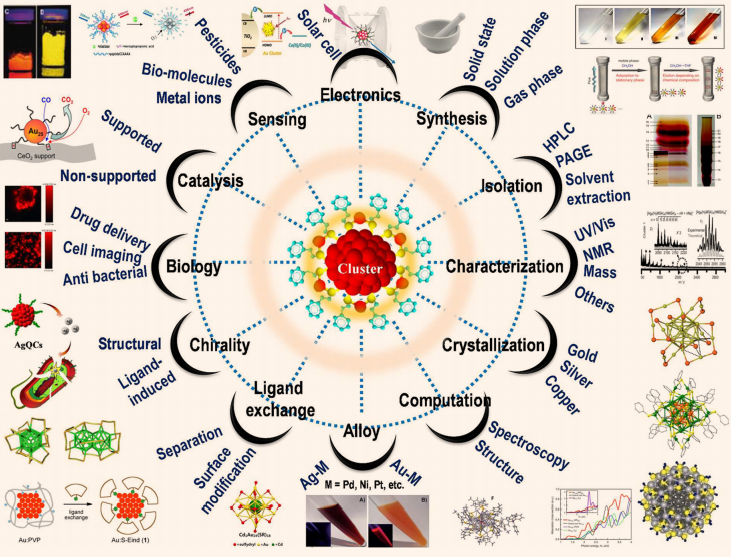
\includegraphics[width=.95\linewidth]{figures/Uses.png}\hfill
            \caption{Schematic representation of different uses for metallic nanoparticles. Wide range of uses and utility of such systems in contemporary technology."Reprinted (adapted) with permission from \cite{BigMNPDiagram}. Copyright 2022 American Chemical Society."}
            \label{Uses}
\end{figure}
%

\section{Introduction}
Mono-, bi-, and poly-metallic nanoparticles (MNPs), or nanoalloys (NAs), find a wealth of potential uses across disciplines ranging from sensing \cite{BioSensors,10.3389/fchem.2020.00341} to drug-delivery,\cite{RAHMAN2021107} memory-storage \cite{https://doi.org/10.1002/nano.202000268,Ditlbacher:00} 
to optics \cite{doi:10.1021/jp026731y,C1NR10788G}.
%
Among the most prominent applications, MNPs further play a significant role as thermal,\cite{doi:10.1021/acs.accounts.8b00521,D0CS00357C,LORBER2022104107} electro-chemical,\cite{C5NR02298C,doi:10.1021/acs.nanolett.9b01523} and photo-chemical \cite{doi:10.1021/acscatal.1c01519,doi:10.1021/ar500411s} catalysts. 
%

The need of a detailed characterization of the MNP's morphology stems from the delicate interplay among size, geometrical features, chemical composition and ordering, and the chemo-physical (e.g., optical, catalytic, etc., etc.) properties of the MNP itself \cite{HotCarrierCreation_Structure,AuPlasmonRev,BioSensors,ExtractHotCars} 
Focusing on catalytic applications, the role of the MNP's and NA's surface is central.
In this context, electronic structure calculations represent an established route to infer the structure-property relationships which rule the activity, selectivity, and stability of the catalyst \cite{Hong2019, Guo2020,Jagannath2018,Chen2021}.
A knowledge of robust structure-property relationships, and of the finite temperature probability of observing MNPs and NAs with a given architecture, in turn, allows to draw design rules, to predict the activity, and to forecast the ageing of a nanocatalysts.

One challenge in such process is the lack of an automated and agnostic characterization of the MNP's and NA's morphology, with a special focus on its surface. 
%
Metallic nanoalloys (NAs) have long been studied for their vast array of promising, novel applications, from biosensors to photovoltaics. Here, we are particularly interested in the optical properties of NAs, combining a plasmonic (gold) and a catalytic (platinum) material for their potential application in plasmon enhanced photo-catalysis \cite{H2Dissociate,MoreH2Dissociate}. Great attention has been paid to the development of such devices as the utilisation of localised surface plasmon resonances (LSPRs) has proven itself a viable and sustainable mean of generating kinetically active electrons and holes (hereafter collectively referred to as hot carriers) for photo-catalytic reactions \cite{HotCarrierCreation_Structure,AuPlasmonRev,BioSensors,ExtractHotCars}. Given current rising concerns as to the sustainability of current sources of energy production, it is critical to provide alternative means of generating and storing energy. It has been widely argued that molecular hydrogen, generated from water splitting, may be used for hydrogen fuel cells--an alternative to contemporary batteries.

To qualitatively understand the nature of the water splitting reaction on AuPt NAs, we look to recent experiments for our design philosophy \cite{JorgeStructure,Anton,RationalDesign}, and adopt their principles of small Pt decorations upon a larger Au seed. This, in principle, ensures that the adsorption surface provided by the Pt is supported atop a larger Au nanoparticle (GNP). The rationale behind this construction being that the Pt may be described as the `fast' component of the cluster, whereas the Au as the `hot'. Respectively, this is because Pt is known to be an excellent catalyst for the water splitting reaction \cite{PtCatalyst}; and that Au has been demonstrated to have strong plasmonic behaviour at incident light wavelengths observed in solar output spectra \cite{AuTRansfer,SolarToChem}.

Whilst it is common and reliable practice to consider many plasmonic effects from a classical perspective, such models assume a sharp cut-off at the boundary of the GNP, in that all contained charges are bound by the surface. Indeed, this is often not the case: electron density can spill out, or tunneling effects between clusters can become effective \cite{PlasmonTunneling}. As such, size dependent shifts of the main plasmon of isolated GNPs or the existence of further surface collective modes that cannot be supported on stepped valence electron distributions are rendered unobtainable via classical models. However, for such nanometric systems, the dynamical many-body quantum mechanical description of LSPRs  may be faithfully captured via time dependent density functional theory (TDDFT) methods. Within the domain of TDDFT, it is often unclear as to what the origin of an observed excitation may be. In one instance, it may indeed be the result of a collective oscillation of the metal's valence electrons, hence being correctly identified as a localised surface plasmon. However, it may also be the case that an observed peak in the absorption spectrum of a cluster is the result of a single electron - hole pair excitation. These are less desirable to generate in a cluster as they will typically recombine monotonically. Whereas, we are instead interested in the Landau damping of an LSPR, which causes the collective oscillation to decay into a pair of hot carriers \cite{ExtractHotCars}. These hot carriers may then be directed from catalytically active sites into an adsorbed molecule. At the size scale considered, it is most likely that observed resonances will correspond to single-pair excitations \cite{SizeLSPR} - especially in the case of Au$_{20}^{Th}$ as the characteristically-large gap between the highest occupied molecular orbital (HOMO), and the lowest unoccupied molecular orbital (LUMO), makes the creation of continuous, and collective excitations prohibitively improbable.

Given the intrinsic quantum mechanical nature of such NAs, and the criticality of determining their plasmocatalytic properties, we have elected to perform a TDDFT study of small AuPt systems - closely monitoring their optical and static properties. It is our intention to demonstrate the profound relationship between the HOMO - LUMO gap, using a nomenclature proper of molecular physics; the distribution of electron orbital characters within the vicinity of the HOMO - LUMO region; and the computed photo-absorption and photo-emission spectra.
%

Au-based nanoalloys, where the Au seed is much larger than the catalytic metal, e.g. Pt, decoration, are the subject of great interest in recent studies. It is understood that the plasmonic properties of the gold seed operating in conjunction with catalytic properties of the other metal may yield a highly efficient photocatalyst.\cite{Cortes2020,Zhang2019}
Among the various catalytic metals to work jointly with Au, Pt has been widely studied. In particular, a lot of attention has been dedicated to Au-core and Pt-shell heterostructures, which have enhanced photocatalytic performance. \cite{Adzic2013,Xia2017} 
These hetereostructures are obtained decorating large Au seed of about 12 $\pm$ 2 nm in diameter with smaller Pt clusters with a diameter of about 2 $\pm$ 1 nm.\cite{Kunwar2019,Engelbrekt2021,Linic2021,Fagan2021} The coinage metal, as Au, is used as a reservoir of hot electrons, accessible to the catalytic component, as Pt.\cite{Xia2017} Such nanoalloys are often characterised by a large optical response before the energy is thermalised into vibrational modes. The thermalisation through electron-phonon coupling seems to depend on the morphology of the nanoparticle.\cite{Staechelin2021} The formation of electron-hole pairs occurs in specific position of the nanoalloy, likely at the plasmonic (Au)/catalytic (Pt)interface. Recent atomistic simulations revealed that the spatial distribution of hot electrons in silver nanoparticles depends on the morphology and the local site.\cite{TRossi2020}
The mechanisms to the flow and extraction of energy and charge carriers, how the plasmon is distributed, where it localises, and its temporal evolution are open challenges in photo(plasmo)catalysis.\cite{Linic2021} 
%
The relative chemical composition of the nanoalloy surface affects strongly the absorption spectra of the AuPt core\@shell,\cite{Rocha2021} while the relative distribution of chemical species within the core influences less the optical properties of the nanoalloy.\cite{Stener2021}
Hence an open challenge is to understand the chemical and structural stability of the decorating catalytic clusters onto a Au seed. Indeed, the Pt loading and shell-thickness of the catalytic material can hinder hot carriers generated in the Au-core to reach the surface.\cite{Jorge2021}
Furthermore, a significant drop of the catalytic performance is likely due to the disappearance of Pt active sites at the surface.\cite{Jorge2019}
%
The chemical ordering of AuPt nanoalloys has been studied mainly on truncated octahedra, thus respecting their bulk FCC layering, and in vacuum.\cite{Divi2016, Jagannath2018,Stener2021} There is a strong evidence that Au atoms surface segregate. This behaviour is in very good agreement with the general trend observed in metallic nanoalloys, where the chemical species with lower surface energy, and larger atomic radius stay preferentially at the nanoalloy surface.\cite{Namsoon2021} 
%
High-resolution transmission electron microscopy (HRTEM) shows the formation of a Pt shell, up to 1-2 layers thick, grown epitaxially onto Au and hence preserving the Au faceting.\cite{Aidan2017}
More and more sophisticated TEM tools boost the numerical search of study aggregation/coalescence of bimetallic systems, where two monometallic nanoparticles, of different materials, hit each other.\cite{Nelli2021}
%
Besides techniques to stabilise a Pt-skin onto an Au-core, choosing specific environment which lowers the Pt-surface energy,\cite{Bian2015} there is experimental evidence that the Pt-decoration(s) are not stable on Au-core and they luckily move underneath Au or coalescence, confirming the best chemical ordering predicted for AuPt. \cite{Hong2019, Guo2020} However, very few calculations have addressed the kinetic rearrangements in AuPt nanolloys in vacuum, but only limited to few cases, in terms of sizes, shapes, and chemical composition.\cite{Jagannath2018,Chen2021}
%
Primarily, this research project is focused on the catalysis of the water splitting reaction on Pt nanoparticles; with the initial design inspired by recent experiments conducted by Salmon et al \cite{JorgeStructure}. That is to say that the adsorption surface provided by the Pt is supported atop a larger Au nanoparticle. The rationale behind this construction being that the Pt may be described as the `fast' component of the cluster, whereas the Au may be described as `hot'. Respectively, this is because Pt is known to be an excellent catalyst for the water splitting reaction \cite{PtCatalyst}; and that Au has been demonstrated to have strong plasmonic behaviour at incident light wavelengths observed in solar output spectra \cite{AuTRansfer,SolarToChem}.

We present the standard operational protocol behind this project. In that we identify a candidate structure which our experimental collaborators are interested in, and we analyse it in both the classical and quauntum mechanical regimes. Respectively, these two scales provide us with insight into the stability of such systems; and the optical performance. Noting that the confluence of these two scales provide us with valuable information regarding their photo-catalytic performance. Having determined a system's efficacy as a plasmon enhanced photo-catalyst, it is our intention for this project to be used to inform and guide the physical creation of systems whose intended purpose is to catalyse the splitting of complex molecules on their surfaces.

In the following report, we shall discuss both nanoparticles and localised surface plasmons, demonstrating the utility of the overlap between the two. We shall then proceed to introduce and motivate the use of density functional theory methods, emerging from quantum mechanical theory; and classical molecular dynamics, a powerful simulation tool, to model systems existing at the nanometric scale. Indeed, we intend to highlight the necessity of adopting a multi-scale modelling approach when  simulating the amazing properties of metallic nanoparticles, a fundamental consideration in this project. We must adopt a systematic approach when describing metallic nanoparticles. With the current state of the art established, the latter three sections of this report will focus on our contributions to this vibrant field of study. We introduce Sapphire, a purpose built platform for designing and analysing metallic nanoparticles which is fast evolving into a dynamical classification tool, whose primary successes include the rapid analysis of multiple characteristics of nanometric structures and of complex surface pattern recognition. We shall then discuss our classical simulations whose stated purpose has been to assess the stability and longevity of composite systems in which a small Pt decoration has been deposited onto a larger Au cluster. Finally, we shall discuss our quantum mechanical calculations of both ground state and excited state properties across a range of geometrical, and chemical isomers. 

Essentially, we are asking the question of ``How much do shape, size, and composition matter when designing a photo-catalyst?''

\section{Background}

\section{Contributions}
\label{s:Contributions}

Our key contributions include:

\begin{enumerate}

  \item Development and deployment of a broad python library for the characterisation and classification of metallic nanoalloys.
  
  \item Exploration of the structure-properties relationship using \textit{ab initio} methods.
  
  \item Studies on the dynamical formation processes of complex nanoalloys.
  
  \item Multi-scale description of light-matter interactions using quantum mechanical and classical models.

\end{enumerate}

\section{Thesis Outline}
\label{s:Outline}

The remainder of this thesis is organized as follows. 

\begin{description}

  \item[Chapter \ref{c:Theory}] provides background information relevant to the field of research. We present the general premise of metallic nanoparticles, the science of plasmonics in both classical and quantum mechanical descriptions, the physics of how plasmons may be used for photo-catalytic purposes, and how metallic nanoparticles may be utilised for the purposes of plasmon enhanced photo-catalysis.
  
  \item[Chapter \ref{c:Sapphire}] details the numerical and analytic methods used to perform the studies carried out in pursuit of this research goal. We present and discuss density functional theory and its time dependent realisations, molecular dynamics from both the \textit{ab initio} and classical perspectives, and theoretical spectroscopic techniques using both classical and quantum mechanical descriptions.
  
  \item[Chapter \ref{c:L-M}] is dedicated to the study of light-matter interactions with respect to metallic nanoparticles. We shall present techniques from \textit{ab-initio} to classical and draw comparrisons between both. Given the nature of this project, understanding how light may interact with nanoparticles is necessary to meeting our research goals. 
  
  \item[Chapter \ref{c:Coal}] details our study into the simulating of various metallic nanoparticle formation processes \textit{in vacuo}. We take inspiration from existing experimental work in an effort to model these dynamic processes. 
  
  \item[Chapter \ref{c:Env}] presents our study into the qualitative description of an interacting environment for our metallic nanoparticles. We present these data and findings to close the narrative on how best to describe our structures in an environment in which they are expected to facilitate the catalysis of specific chemical reactions.
  
  \item[Chapter \ref{c:Conclusions}] concludes this thesis. We shall present the core principles of the research carried out - re-establishing the central narrative of the beauty at the nanoscale. Following this, we shall illuminate interesting aspects which require a broader scope with respect to the work to appreciate sufficiently. Finally, we shall provide a thorough discussion of future research which may arise from our findings and investigations herein.
  
\end{description}



